\documentclass[12pt, twoside]{article}
\usepackage[letterpaper, margin=1in, headsep=0.5in]{geometry}
\usepackage[english]{babel}
\usepackage[utf8]{inputenc}
\usepackage{amsmath}
\usepackage{amsfonts}
\usepackage{amssymb}
\usepackage{tikz}
\usetikzlibrary{quotes, angles}
\usepackage{graphicx}
\usepackage{enumitem}
\usepackage{multicol}

\newif\ifmeta
\metatrue %print standards and topics tags

\title{Regents Geometry}
\author{Chris Huson}
\date{November 2021}

\usepackage{fancyhdr}
\pagestyle{fancy}
\fancyhf{}
\renewcommand{\headrulewidth}{0pt} % disable the underline of the header
\raggedbottom


\fancyhead[LE]{\thepage}
\fancyhead[RO]{\thepage \\ Name: \hspace{4cm} \,\\}
\fancyhead[LO]{BECA / Dr. Huson / Geometry 04 Analytic Geometry}

\begin{document}

\subsubsection*{4.11 Linear functions}
\begin{enumerate}
\item Do Now: A linear equation $f$ is graphed below.
\begin{multicols}{2}
\begin{enumerate}
  \item State the coordinates of the point $A$. \vspace{0.25cm}
  \item Write down the line's slope.\\ $m=$
  \vspace{0.25cm}
  \item Write down it's $y$-intercept.\\ $b=$
  \vspace{0.25cm}
  \item Write down the equation of the line.
  \vspace{1cm}
  \item Find the $x$-intercept.
\end{enumerate} \vspace{.5cm}
  \begin{center} 
  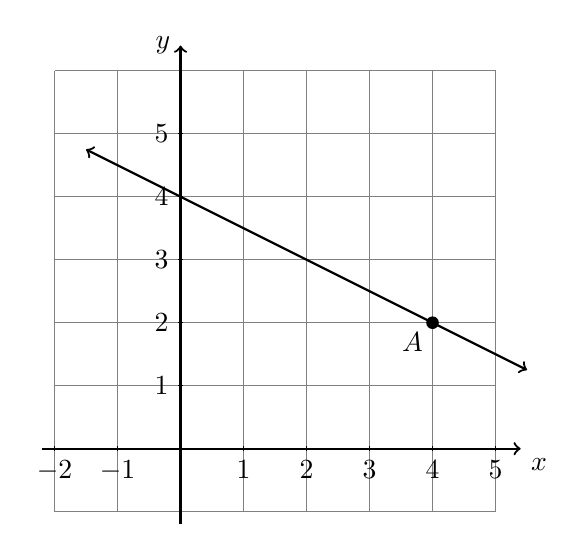
\begin{tikzpicture}[scale=0.8]
    \draw [help lines] (-2,-1) grid (5,6);
    \draw [thick, ->] (-2.2,0) -- (5.4,0) node [below right] {$x$};
    \draw [thick, ->] (0,-1.2)--(0,6.4) node [left] {$y$};
    \foreach \x in {-2,-1,1,2,...,5} \draw (\x cm,1pt) -- (\x cm,-1pt) node[anchor=north] {$\x$};
    \foreach \y in {1, 2, 3, 4, 5} \draw (1pt,\y cm) -- (-1pt,\y cm) node[anchor=east] {$\y$};
    \draw [thick, <->] (-1.5,4.75) -- (5.5,1.25);
    \fill (4,2) circle[radius=0.1] node[below left]{$A$};
  \end{tikzpicture}
  \end{center}
\end{multicols} \vspace{1cm}


\item Two lines are graphed below. 
\begin{enumerate}
  \item Complete the T-tables for each.
  \item Write down the equations for each.
\end{enumerate}
  \begin{center} 
  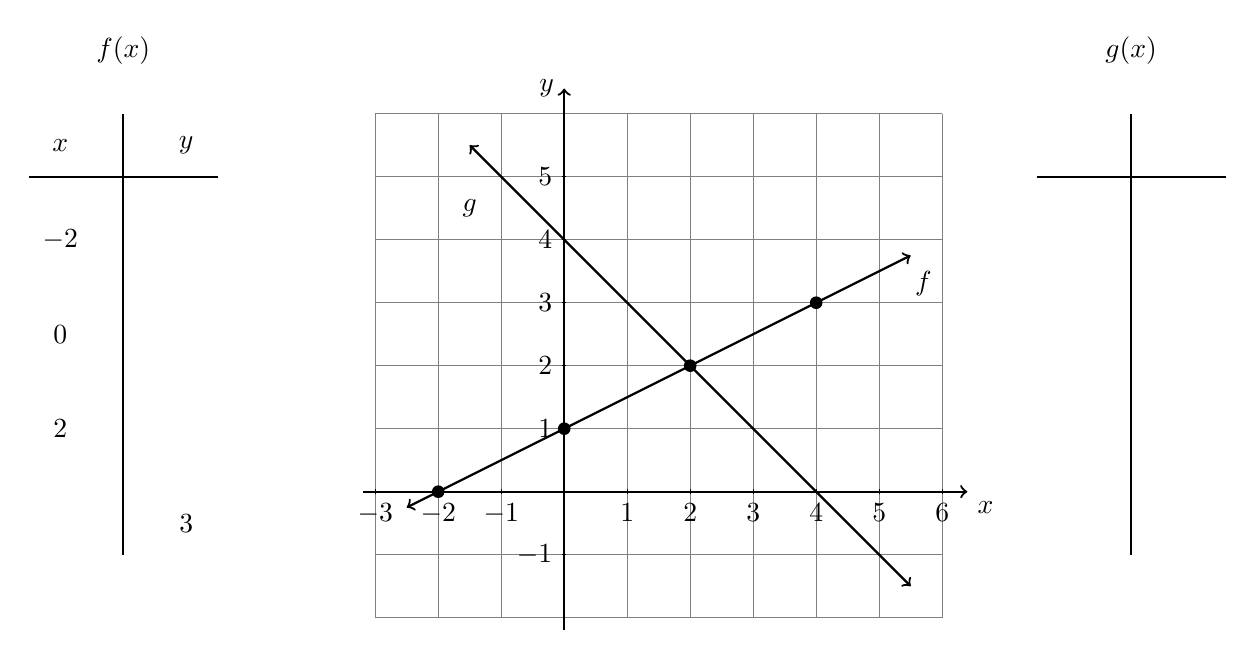
\begin{tikzpicture}[scale=0.8]
    \draw [help lines] (-3,-2) grid (6,6);
    \draw [thick, ->] (-3.2,0) -- (6.4,0) node [below right] {$x$};
    \draw [thick, ->] (0,-2.2)--(0,6.4) node [left] {$y$};
    \foreach \x in {-3,-2,-1,1,2,...,6} \draw (\x cm,1pt) -- (\x cm,-1pt) node[anchor=north] {$\x$};
    \foreach \y in {-1,1, 2, 3, 4, 5} \draw (1pt,\y cm) -- (-1pt,\y cm) node[anchor=east] {$\y$};

    \draw [thick, <->,samples=20,domain=-2.5:5.5] plot(\x,0.5*\x+1);
    \node at (5.7,3.3){$f$};
    \draw [thick, <->,samples=20,domain=-1.5:5.5] plot(\x,-1*\x+4);
    \node at (-1.5,4.5){$g$};

    \draw [thick] (-7,-1) -- (-7,6);
    \draw [thick] (-8.5,5) -- (-5.5,5);
    \node at (-7,7){$f(x)$};
    \node at (-8,5.5){$x$};
    \node at (-6,5.5){$y$};
    \draw [thick] (9,-1) -- (9,6);
    \draw [thick] (7.5,5) -- (10.5,5);
    \node at (9,7){$g(x)$};
    \node at (-8,4){$-2$}; 
    \node at (-8,2.5){$0$}; 
    \node at (-8,1){$2$}; 
    \node at (-6,-0.5){$3$};
    \fill (-2,0) circle[radius=0.1];
    \fill (0,1) circle[radius=0.1];
    \fill (2,2) circle[radius=0.1];
    \fill (4,3) circle[radius=0.1];
  \end{tikzpicture}
  \end{center}

\newpage
\item A function is defined as $f(x)=2x+3$. Find each value.
\begin{enumerate}
  \begin{multicols}{2}
  \item $f(4)=$ 
  \vspace{0.5cm}
  \item $f(0)=$
  \vspace{0.5cm}
  \item $f(-3)=$
  \vspace{0.5cm}
  \item $f(1)=$
\end{multicols}\vspace{0.5cm}
  \item Find the value of $x$ that makes $f(x)=0$
\end{enumerate} \vspace{2cm}

\subsubsection*{Point-slope form: $(y-y_1)=m(x-x_1)$}
\item Write the linear equation $y-1=2(x-3)$ in the form $y=mx+c$. \vspace{4cm}

\item A line has a gradient (slope) of $\displaystyle \frac{3}{4}$ and passes through the point $(8, 3)$. Find the equation of the line in the form $y=mx+b$.
\vspace{4cm}

\item Find the equation of the line through the points $(1, 3)$ and $(5, 4)$. 


\end{enumerate}
\end{document}